\chapter{I Sensori e il loro utilizzo per ottenere Interazioni Implicite}

Come detto in precedenza una delle funzionalità principali dell'applicazione è riconoscere come l'utente si sta spostando in un determinato momento e, in questa fase dello sviluppo, ci siamo concentrati nel costruire un sistema che deducesse in modo autonomo se un'utente si trova alla guida o meno. Di seguito si spiegherà come questo scopo è stato raggiunto attraverso il lavoro coordinato di vari sensori.


\section{I sensori}
In GeneroCity un sensore è un modulo software\footnote{La programmazione modulare è un paradigma di programmazione che consiste nella realizzazione di programmi suddivisi in moduli, ognuno dei quali svolge precise funzioni.} che analizza il contesto in cui si trova l'utente in uno specifico istante per determinare l'azione compiuta da quest'ultimo. In particolare ciascuno di essi calcola un valore reale compreso tra 0 e 1, detto \textbf{confidenza}, il quale rappresenta il grado di sicurezza con il quale il sensore ha effettuato la rilevazione del'azione (dove 0 rappresenta una sicurezza minima e 1 massima). Poiché nella versione attuale dell'applicazione l'azione che viene rilevata è solamente una, possiamo approssimare la confidenza come la probabilità che l'utente stia guidando. Più specificamente:
\begin{itemize}
    \item un valore compreso tra 0 e 0,5 (stato \textit{walking}) indica che l'utente non sta guidando;
    \item il valore 0,5 (stato \textit{unknown}) denota che il sensore non è in grado di inferire lo stato dell'utente;
    \item una confidenza compresa tra 0,5 e 1 (stato \textit{automotive}) segnala che l'utente sta guidando.
\end{itemize}

Per analizzare il contesto e calcolare la confidenza ogni sensore può adottare svariati approcci: esso si può basare sulle rilevazioni di un vero e proprio sensore (come quelli di movimento o ambientali), sullo stato di una specifica componente del dispositivo, ad esempio la batteria o il display, oppure può far uso della connettività Wi-Fi, Bluetooth o utilizzare altre tecnologie e protocolli specifici, come la geolocalizzazione attraverso GPS. Una linea guida importante per lo sviluppo di un sensore è che esso si avvalga una sola di queste tecnologie o componenti in modo da effettuare la computazione in maniera indipendente dagli altri: ad esempio non succederà mai che il sensore Bluetooth effettui una scansione dei dispositivi vicini quando il GPS rileva che l'utente si sta muovendo ad una certa velocità. Questo perché sarà l'insieme dei risultati ottenuti da tutti i sensori a concorrere al calcolo dell'effettivo stato dell'utente ed eventuali correlazioni tra sensori differenti verranno prese in considerazione dal sistema durante questa computazione tramite apprendimento automatico.


\section{Il flusso di aggiornamento della confidenza in GeneroCity Android}
Dato che i sensori sono molteplici un fattore importante è la loro coordinazione: lo stato dell'utente sarà determinato basandosi sulla confidenza di ogni sensore ed è quindi importante che esso sia aggiornato ogni qualvolta un sensore cambia la sua confidenza. Per sincronizzare il lavoro dei sensori è stato quindi fondamentale definire delle funzionalità comuni che ogni sensore deve avere. Questo è stato possibile sfruttando il paradigma di programmazione orientata agli oggetti implementato in Java\cite{ref:Java}, in particolare è stata definita una classe astratta\footnote{Nella programmazione orientata agli oggetti una classe astratta è una classe che non può essere istanziata, la quale definisce delle funzionalità di base per tutte le sue sotto classi.} che tutti i sensori ereditano.

\subsection{La classe astratta Sensor}
Ogni sensore eredita dalla classe Sensor i seguenti attributi: il \textit{nome} univoco che identifica il sensore, la \textit{versione} del sensore, il \textit{peso} (rappresentato come numero reale) che ha il sensore nel calcolo dello stato dell'utente.

Inoltre ogni sensore mantiene uno storico della confidenza che ha calcolato tramite una mappa ad albero\footnote{Una treemap è una struttura dati che implementa le funzionalità di normale una normale mappa, ossia immagazzina delle coppie (chiave, valore), e inoltre mantiene l'ordinamento delle coppie basato sull'ordinamento naturale delle chiavi.} che adotta come chiave lo Unix Timestamp\footnote{Lo Unix Timestamp rappresenta il numero di secondi trascorsi dalla mezzanotte del 1° Gennaio 1970.} del momento in cui il valore è stato calcolato. Di seguito vengono riportati i principali metodi esposti da questa classe.
\subsubsection{getStatus}
\begin{minted}[
framesep=2mm,
linenos,
breaklines
]{java}
public abstract double getStatus(Calendar timestamp);
\end{minted}
Esso ha come parametro un Timestamp e restituisce la confidenza del sensore calcolata nell'istante più vicino a quello passato come parametro. Questo metodo è l'unico metodo astratto ed è quindi il metodo principale che i sensori concreti dovranno implementare.
\subsubsection{update}

\begin{minted}[
framesep=2mm,
linenos,
breaklines
]{java}
public void update(Calendar timestamp, SensorData sensorData) {
    collect(timestamp, sensorData);
    GCSensorConstants.onUpdate(timestamp);
}
\end{minted}
Il metodo update riceve in input un Timestamp e un oggetto di un tipo da noi definito, denominato SensorData, contenente i dati inviati dal sensore. Questo metodo si occuperà di inviare i dati raccolti al server, attraverso il metodo \textit{collect}, e di innescare il ricalcolo dello stato dell'utente.
Quando viene eseguito il metodo update viene notificata l'unità centrale: una classe statica chiamata SensorConstants. Essa, attraverso il metodo \textit{onUpdate}, richiede lo stato di ogni sensore (utilizzando il metodo getStatus) e calcola il nuovo stato dell'utente attraverso il metodo \textit{compute}. Attualmente questo stato viene rappresentato come la media pesata delle confidenza di ogni sensore in uno specifico momento.

\subsubsection{GCSensorConstants.onUpdate}
\begin{minted}[
framesep=2mm,
linenos,
breaklines
]{java}
static void onUpdate(Calendar time) {
    if (updating) {
        return;
    }

    updating = true;
    double computed = compute(time);
    computeHistory.put(time.getTimeInMillis(), computed);
    updating = false;
}
\end{minted}

\subsubsection{GCSensorConstants.compute}
\begin{minted}[
framesep=2mm,
linenos,
breaklines
]{java}
private static double compute(Calendar time) {
    double sum = 0.0;
    double wei = 0.0;

    double confidence;
    for (GCSensorInterface module : sensors) {
        confidence = module.getStatus(time);

        sum += (confidence - 0.5d) * module.weight;
        wei += module.weight;
    }

    return sum / wei + 0.5d;
}
\end{minted}

\subsection{L'invio di dati al server}
Come anticipato ogni qualvolta viene aggiornata la confidenza di un sensore il metodo update richiede in input un oggetto di tipo SensorData che rappresenta lo stato del sensore al momento dell'aggiornamento. Questo perché, prima che venga ricalcolata la confidenza media, viene chiamato il metodo \textit{collect} che serializza l'oggetto in formato JSON e lo invia al server tramite una richiesta HTTP all'endpoint in figura \ref{fig:endpoint}, il quale si occuperà di memorizzare i dati forniti dal sensore nel database. Questi dati vengono mantenuti al fine sia di tenere traccia del corretto funzionamento dei sensori, sia perché verranno utilizzati per l'allenamento di un modello di Machine Learning che verrà implementato in futuro in GeneroCity per determinare lo stato dell'utente.

\begin{figure}[h]
    \centering
    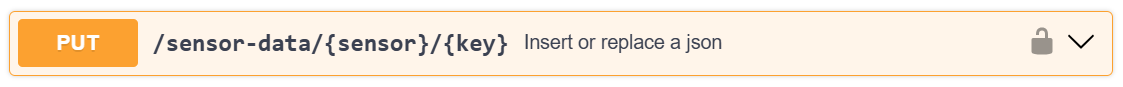
\includegraphics[width=1\linewidth]{images/endpoint.png}
    \caption{L'endpoint chiamato per memorizzare i dati dei sensori sul database}
    \label{fig:endpoint}
\end{figure}

\subsubsection{collect}
\begin{minted}[
framesep=2mm,
linenos,
breaklines
]{java}
public void collect(Calendar timestamp, SensorData sensorData) {
    long tsMillis = timestamp.getTimeInMillis();
    if (tsMillis - lastApiTimestamp <= getApiCooldownMs()) {
        return;
    }

    lastApiTimestamp = tsMillis;
    String key = ver + "-" + app.config().getMyId() + "-" + timestamp.getTimeInMillis();
    app.api().setSensorData(name, key, sensorData).enqueue(updateCall);
}
\end{minted}
La classe SensorData serializza le seguenti informazioni:
\begin{itemize}
    \item \textit{datetime}: la data e l'ora in cui è avvenuto l'aggiornamento seguendo il formato definito nello standard RFC3339\cite{ref:RFC3339};
    \item \textit{confidence}: la confidenza calcolata dal sensore al momento dell'aggiornamento;
    \item \textit{action}: l'azione che il sensore ha rilevato (\textit{walking}, \textit{unknown} o \textit{automotive});
    \item \textit{data}: alcuni dati aggiuntivi specifici del sensore che ha effettuato la rilevazione, i quali indicano lo stato in cui si trovava il sensore. Ad esempio per il sensore Wi-Fi questi dati possono essere relativi alla rete a cui il dispositivo è connesso, mentre per il sensore GPS le coordinate geografiche in cui l'utente si trova.
\end{itemize}
Di seguito un esempio di body inviato dal sensore bluetooth attraverso una richiesta HTTP:
\begin{minted}[
framesep=2mm,
linenos,
breaklines
]{json}
{
   "action":"automotive",
   "confidence":0.75436,
   "data":{
      "connected":[
         {
            "alias":"My Car",
            "bluetooth_class":"Handsfree",
            "connection_count":4,
            "device_name":"Fiat Punto",
            "is_car":true
         }
      ],
      "bluetooth_enabled":true
   },
   "datetime":"2024-10-21T15:43:24.525+02:00"
}
\end{minted}
Come si può notare il campo data è costruito sulla base dello stato del sensore: in particolare si evince che il bluetooth è attivo e il dispositivo è connesso ad un dispositivo che viene identificato come macchina.

In aggiunta a questi dati nel path della richiesta (figura \ref{fig:endpoint}) vengono anche mandati il nome del sensore utilizzato ed una chiave univoca usata per identificare la richiesta nel database. Essa è costruita utilizzando la versione del sensore, l'id dell'utente autenticato nell'applicazione ed il Timestamp del momento in cui viene inviata la richiesta.

Inoltre, onde evitare un sovraccarico del server, è stato definito un tempo di \textit{cooldown} tra le richieste: ogni volta che viene notificato un aggiornamento da parte del sensore, se questo tempo non è trascorso dall'ultima richiesta, allora la richiesta viene scartata ma viene comunque ricalcolata la nuova media.

\section{Il compito del sensore Bluetooth}
La quasi totalità delle automobili prodotte al giorno d'oggi hanno installata un'autoradio dotata di tecnologie bluetooth, dando la possibilità ai guidatori di riprodurre musica, effettuare chiamate o utilizzare software come Android Auto o Apple Car Play per sfruttare alcune funzionalità dello smartphone durante la guida.\cite{ref:car-bluetooth} L'obiettivo del mio tirocinio è stato aggiungere al sistema precedentemente descritto un sensore bluetooth in grado di capire se l'utente sta conducendo un veicolo. Esso dovrà restituire un valore di confidenza adeguato calcolato sulla base dei dispositivi connessi allo smartphone di quest'ultimo tramite la medesima tecnologia.

Prima di integrare questa nuova funzionalità in GeneroCity si è scelto di sviluppare una piccola applicazione a sé stante allo scopo di prendere dimestichezza con l'SDK\footnote{Acronimo che sta per Software Development Kit, ossia un'insieme di strumenti per lo sviluppo del software} di Android per Java, nello specifico con le sue funzionalità riguardanti la connettività via bluetooth.
